\phantomsection\numberedsection{RF5.1 Crear relación}

\subsection*{Descripción}
Permite a los usuarios definir nuevas relaciones para poder relacionar los productos y sugerirlos de una forma más rápida.\par
\vspace{0.15cm}

\textbf{Pre-condición}\par
El usuario debe de tener la sesión iniciada en Mini PIM.\par
\vspace{0.15cm}

\textbf{Post-condición}
\begin{itemize}
    \item Caso de éxito: La relaciones creada correctamente, se muestra en la lista de relaciones con el nombre ingresado y el contador de productos asociado inicia en cero.
    \item Caso mínimo: El sistema notifica al usuario el resultado de la acción de crear relación: exitosa o fallida.
\end{itemize}

\textbf{Prioridad: }
Alta
\vspace{0.15cm}

\textbf{Autor: }
Pablo Ortega Serapio y Francisco Javier Jordá Garay\par
\vspace{0.15cm}

\textbf{Control de cambios: } Versión 1: Definición del caso de uso

\numberedsubsection{Escenario principal}
\begin{enumerate}
    \item El usuario accede a la sección de gestión de relaciones.
    \item El sistema valida que el número total de relaciones creadas por el usuario es menor que el límite establecido en el plan gratuito
    \item El sistema muestra la lista de relaciones existentes y la opción para crear una nueva.
    \item El usuario selecciona la opción para crear una nueva relación.
    \item El sistema muestra el menú de creación de relación.
    \item El usuario ingresa el nombre deseado y confirma la creación de la relación.
    \item El sistema verifica que el nombre de la relación no esté vacío.
    \item El sistema crea la nueva relación y actualiza la lista de relaciones para incluirla.
    \item El usuario visualiza la nueva relación en la lista, con el nombre ingresado y un contador de productos asociados que empieza en cero.
\end{enumerate}

\numberedsubsection{Escenarios alternativos}
\begin{description}

    \item[3.a] El sistema no permite crear relaciones.
    \begin{enumerate}
        \item[3.a.1] El sistema no permite crear relaciones adicionales hasta que una vez hecha la comprobación vea que no tiene el numero máximo de relaciones creadas.
    \end{enumerate}

    \item[5.a] El usuario cancela la acción de crear una relación nueva seleccionando la opción que cierra el menú.
    \begin{enumerate}
        \item[5.a.1] El sistema regresa a la sección de gestión de relaciones
    s de los datos.
    \end{enumerate}

    \item[7.a] El sistema detecta que el nombre de la relación es erróneo\footnote{Se considera erróneo cualquier nombre que este vacío, no sea único o sea igual a algún GTIN o algún SKU del sistema}.
    \begin{enumerate}
        \item[7.a.1] El sistema muestra un mensaje de error solicitando un nombre válido.
        \item[7.a.2] El sistema devuelve al usuario a la pestaña para seguir creando la relación.
    \end{enumerate}
\end{description}

\numberedsubsection{Casos de Prueba}
\underline{Escenario: Principal}\par
\vspace{0.15cm}
\textbf{Dado} que he iniciado sesión con mi cuenta de usuario correspondiente,\par
\textbf{Y} estoy en el apartado de relaciones,\par
\textbf{Y} el sistema comprueba que no tengo el número máximo de relaciones creadas,\par
\textbf{Cuando} selecciono la opción de \enquote{Añadir relación},\par
\textbf{E} introduzco correctamente el nombre de la relación que deseo crear,\par
\textbf{Y} selecciono \enquote{Confirmar} para guardar los datos,\par
\textbf{Entonces} el sistema almacena la información de la nueva relación en la base de datos del Mini PIM,\par
\textbf{Y} actualiza la lista de relaciones con la nueva relación creada,\par
\textbf{Y} muestra el apartado de relaciones con todas las relaciones almacenadas, incluyendo la nueva con un contador de productos en cero.\par

\vspace{0.20cm}



\underline{Escenario: Alternativo 3.a}\par
\vspace{0.15cm}

\textbf{Dado} que he iniciado sesión con mi cuenta de usuario correspondiente,\par
\textbf{Cuando} accedo al apartado de relaciones,\par
\textbf{Y} el sistema verifica que tengo el numero máximo de relaciones creadas,\par
\textbf{Entonces} el sistema no me permite pulsar el botón para crear una nueva relación,\par
\textbf{Y} no me permite crear más relaciones hasta que verifique que no tengo el numero máximo de relaciones.\par
\vspace{0.20cm}

\underline{Escenario: Alternativo 5.a}\par
\vspace{0.15cm}

\textbf{Dado} que he iniciado sesión con mi cuenta de usuario correspondiente,\par
\textbf{Y} estoy en el apartado de relaciones,\par
\textbf{Y} el sistema comprueba que no tengo el número máximo de relaciones creadas,\par
\textbf{Cuando} selecciono la opción de \enquote{Añadir relación},\par
\textbf{Y} selecciono la opción de cancelar o cerrar el menú de creación sin ingresar ningún nombre,\par
\textbf{Entonces} el sistema regresa a la sección de gestión de relaciones,\par
\textbf{Y} muestra el apartado de relaciones sin ningún cambio.\par

\vspace{0.20cm}

\underline{Escenario: Alternativo 7.a}\par
\vspace{0.15cm}

\textbf{Dado} que he iniciado sesión con mi cuenta de usuario correspondiente,\par
\textbf{Y} estoy en el apartado de relaciones,\par
\textbf{Y} el sistema comprueba que no tengo el número máximo de relaciones creadas,\par
\textbf{Cuando} selecciono la opción de \enquote{Añadir relación},\par
\textbf{Y} relleno el campo de nombre de la relación de forma errónea,\par
\textbf{Entonces} el sistema me notifica que el campo de nombre es erróneo,\par
\textbf{Y} muestra un mensaje de error y me devuelve al apartado de relaciones sin ningún cambio.\par

\vspace{0.20cm}

\numberedsubsection{Bocetos}
\begin{figure}[H]
    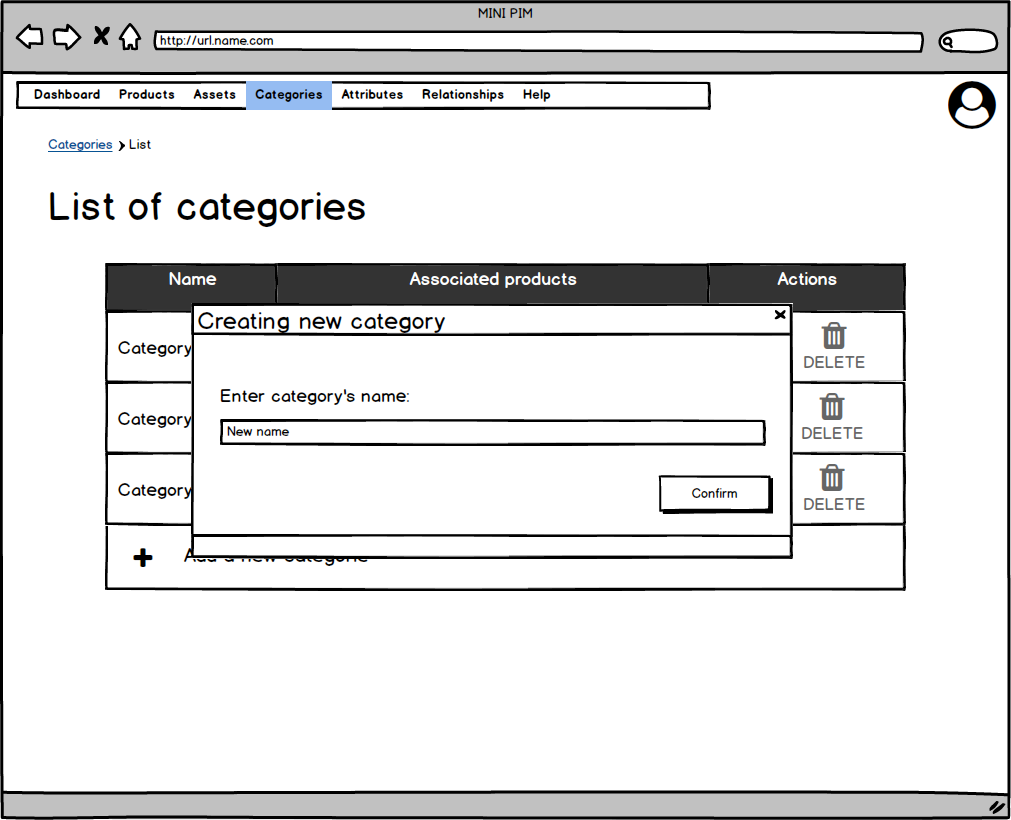
\includegraphics[width=1\linewidth]{mockups/RF4.1_1.png}
    \caption{Creación de relación
}
   \end{figure}
\vspace{1.0cm}

\begin{figure}[H]
    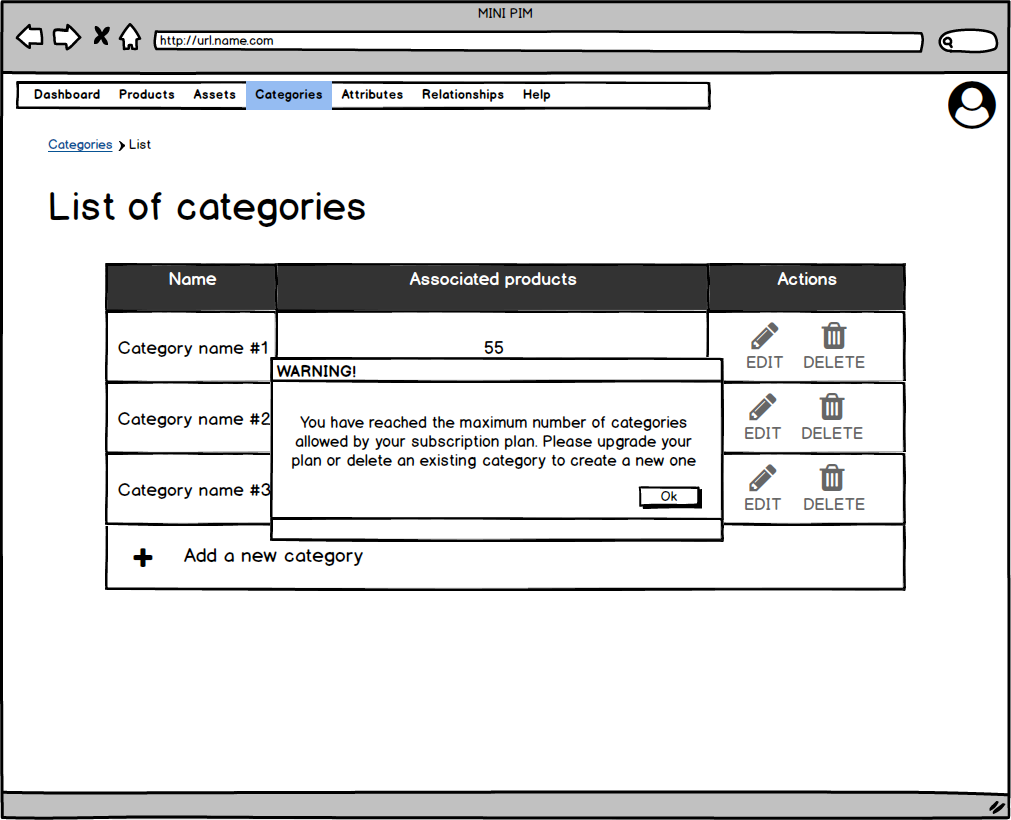
\includegraphics[width=1\linewidth]{mockups/RF4.1_2.png}
    \caption{Error por llegar al máximo de relación
s}
   \end{figure}
\vspace{1.0cm}

\newpage % Nuevo caso de uso en nueva página